\scanpage{285}

\[
\begin{aligned}
gaU&=g'aU\quad\text{si }gU=g'U\ \text{i.e.}\quad g'^{-1}g\in U\\
a^{-1}(g'^{-1}g)a\deleted{U}&\in U\quad\text{si }g'^{-1}g\in U\\
&a^{-1}Ua
\end{aligned}
\]

\figure{\begin{tikzpicture}[x=0.008cm,y=-0.008cm]
\draw (0,0)--(90,47)--(86,148);
\end{tikzpicture}}

\[
x\qquad\lambda x
\]

\figure{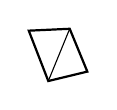
\begin{tikzpicture}[x=0.008cm,y=-0.008cm]
\draw[thick] (0,0)--(65,-3)--(93,65)--(31,80)--cycle;
\draw (31,80)--(65,-3);
\end{tikzpicture}}

\figure{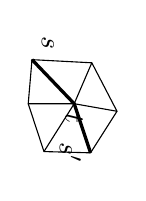
\begin{tikzpicture}[x=0.008cm,y=-0.008cm]
\draw (0,0)--(95,5)--(135,82)--(93,148)--(19,146)--(-6,70)--cycle;
\draw[very thick] (0,0)--(67,70)--(93,148);
\draw (95,5)--(67,70)--(19,146);
\draw (-6,70)--(67,70)--(135,82);
\node[above left,rotate=-90] at (0,0) {$s$};
\node[right,rotate=-90] at (67,70) {$t$};
\node[below,rotate=-90] at (93,148) {$s'$};
\end{tikzpicture}}

\[
\begin{aligned}
\underset{\substack{\shortparallel\\ B}}{G_{\unsure{x_0|s_0}}}
=G_s=\underset{\substack{\shortparallel\\\mathrm{int}(g)\,B}}{G_{g\cdot s_0}}
\end{aligned}
\]

\figure{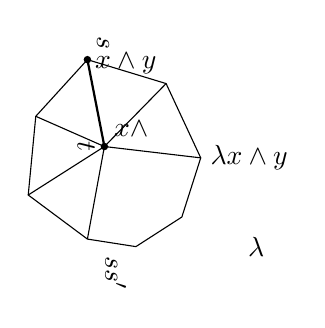
\begin{tikzpicture}[x=0.008cm,y=-0.008cm]
\draw (100,0)--(225,38)--(280,156)--(250,250)--(177,297)--(100,285)--(6,215)--(18,90)--cycle;
\draw[thick] (100,0)--(127,138);
\draw (225,38)--(127,138)--(280,156);
\draw (18,90)--(127,138)--(100,285);
\draw (6,215)--(127,138);
\fill (100,0) circle[radius=1.35pt];
\fill (127,138) circle[radius=1.35pt];
\node[above left,rotate=-90] at (100,0) {$s$};
\node[below,rotate=-90] at (127,138) {$t$};
\node[below right,rotate=-90] at (177,297) {$\deleted{\unsure{s}}s'$};
\node[above left] at (225,38) {$x\wedge y$};
\node[above right] at (127,138) {$\deleted{x\wedge}$};
\node[right] at (280,156) {$\deleted{\lambda x\wedge y}$};
\node[right=13mm] at (177,297) {$\lambda$};
\end{tikzpicture}}

\[
\begin{aligned}
x\wedge y=e&\Rightarrow x\wedge\overbrace{\lambda y}^{y'}=\lambda e\\
&\lambda^{-1}x\wedge y'=e
\end{aligned}
\]

\figure{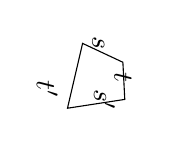
\begin{tikzpicture}[x=0.008cm,y=-0.008cm]
\draw (24,0)--(88,30)--(91,89)--(0,103)--cycle;
\node[above,rotate=-90] at (24,0) {$s$};
\node[right,rotate=-90] at (88,30) {$t$};
\node[below,rotate=-90] at (91,89) {$s'$};
\node[below left,rotate=-90] at (0,103) {$t'$};
\end{tikzpicture}}

\figure{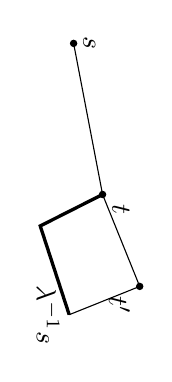
\begin{tikzpicture}[x=0.008cm,y=-0.008cm]
\draw (53,-240)--(99,0)--(158,146)--(46,191);
\draw[very thick] (46,191)--(0,50)--(99,0);
\fill (53,-240) circle[radius=1.35pt];
\fill (99,0) circle[radius=1.35pt];
\fill (158,146) circle[radius=1.35pt];
\node[above,rotate=-90] at (53,-240) {$s$};
\node[above right,rotate=-90] at (99,0) {$t$};
\node[below right,rotate=-90] at (158,146) {$t'$};
\node[below,rotate=-90] at (46,191) {$\lambda^{-1}s$};
\end{tikzpicture}}

\figure{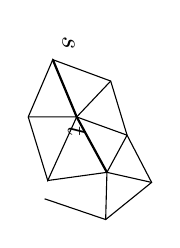
\begin{tikzpicture}[x=0.008cm,y=-0.008cm]
\draw (32,0)--(124,34)--(150,120)--(189,195)--(116,254)--(19,221);
\draw (-7,91)--(32,0)--(70,91)--(124,34);
\draw (-7,91)--(70,91)--(150,120)--(118,179)--(189,195);
\draw[thick] (32,0)--(70,91)--(118,179);
\draw (-7,91)--(24,192)--(70,91);
\draw (24,192)--(118,179)--(116,254);
\node[above left,rotate=-90] at (32,0) {$s$};
\node[right,rotate=-90] at (70,91) {$t$};
\end{tikzpicture}}

\figure{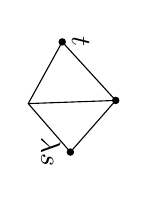
\begin{tikzpicture}[x=0.008cm,y=-0.008cm]
\draw (54,0)--(139,93)--(67,175)--(0,98)--cycle;
\draw (0,98)--(139,93);
\fill (54,0) circle[radius=1.35pt];
\fill (139,93) circle[radius=1.35pt];
\fill (67,175) circle[radius=1.35pt];
\node[above,rotate=-90] at (54,0) {$t$};
\node[below,rotate=-90] at (67,175) {$\lambda s$};
\end{tikzpicture}}

\[
\begin{aligned}
\underset{\shortparallel}{\mathrm{Et}_{A_0}(s)}&\xrightarrow{\lambda}\mathrm{Et}_{A_0}(\lambda^{-1}s)\\
\{y\mid x\wedge y=e\}&\qquad\{y'\mid\lambda^{-1}x\wedge y'=e\quad\text{i.e. }x\wedge y'=\lambda e\}\\
&y\longmapsto y'=\lambda y
\end{aligned}
\]

\figure{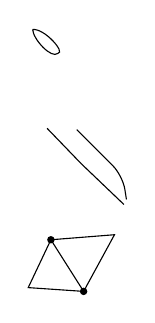
\begin{tikzpicture}[x=0.008cm,y=-0.008cm]
\draw (0,0) .. controls (19,-2) and (53,37) .. (40,38) .. controls (30,47) and (1,16) .. (0,0);
\draw[rounded corners=5pt] (70,159)--(143,232)--(149,270);
\draw (23,157)--(77,213);
\draw (77,213)--(145,278);
\draw (29,334)--(130,326)--(81,416)--(-7,410)--cycle;
\draw (29,334)--(81,416);
\fill (29,334) circle[radius=1.35pt];
\fill (81,416) circle[radius=1.35pt];
\end{tikzpicture}}

\[
{\rho}^{-1}(u)\,\rho^{-1}(a^{-1})\,a^{-1}
\]

\[
\begin{aligned}
y&\longmapsto y+x &\deleted{\lambda\unsure{v|x}}\quad y_1&=y+x\\
y'&\longmapsto y'+\lambda^{-1}x &\deleted{y'_1=y'+\lambda}&\\
&&\underset{y'_1}{\underline{\lambda y_1}}&=\underset{y'}{\underline{\lambda y}}+\lambda x=\\
&&y'_1&=y'+\lambda^2(\lambda^{-1}x)
\end{aligned}
\]

\figure{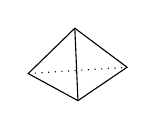
\begin{tikzpicture}[x=0.008cm,y=-0.008cm]
\draw (0,72)--(74,0)--(157,62)--(79,115)--cycle;
\draw (74,0)--(79,115);
\draw[dotted] (0,72)--(157,62);
\end{tikzpicture}}

\[
\begin{aligned}
\unsure{\rho_\infty|\beta_\infty|\rho_0}U&=h_\infty U & \tau_0\ \tau_1\\
h_\infty^{-1}\tau_0&\in U &\tau_1\\
\tau_0\underset{h_\infty}{\underbrace{\tau_1\tau_0}}&\in\underset{\substack{\shortparallel\\\langle\tau_1,\tau_{\unsure{2|\infty}}\rangle}}{U} &\mathrm{Et}(s)&=\\
\tau_0\tau_1\tau_0&\quad\therefore
\end{aligned}
\]

\[
\begin{aligned}
(s,t)&\qquad s,t &\{s,t\}\in A_0&\Longleftrightarrow\{s,\lambda t\}\in A_\lambda\\
\mathrm{Et}_{A_0}(t)&=\mathrm{Et}_{A_\lambda}(\lambda t) &&\mathrm{Et}(s)\cap\mathrm{Et}(\lambda t)
\end{aligned}
\]

\[
\begin{aligned}
\{s,\deleted{\unsure{\lambda}}t\}&\in A_0 &(s,t)&\in A_\lambda\\
\{s,\lambda^{-1}u\}&\in A_0 &(s,u\}&\in A_\lambda\\
\{t,\lambda^{-1}u\}&\in A_0 &(t,u)&\in A_\lambda
\end{aligned}
\]

\figure{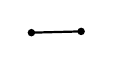
\begin{tikzpicture}[x=0.008cm,y=-0.008cm]
\draw[thick] (0,0)--(79,-2);
\fill (0,0) circle[radius=1.35pt];
\fill (79,-2) circle[radius=1.35pt];
\end{tikzpicture}}

% archive sheet number: 284
